\documentclass[12pt]{iptex}
% IDIOMA
% Se necessário, inserir línguas e indicar língua principal (main)
\usepackage[main=brazil,english]{babel}
\usepackage[italic]{mathastext}
\sisetup{
    group-separator={.},
    group-minimum-digits=3,
    output-decimal-marker={,}}

% Alterando nome do TOC (adicionar em outras línguas, se necessário)
\addto\captionsbrazil{%
	\renewcommand{\contentsname}{SUMÁRIO}
	\renewcommand{\refname}{REFERÊNCIAS}
}

% BIBLIOGRAFIA
%\usepackage[abnt-emphasize=bf,alf]{abntex2cite}
% Para bibliografia ABNT com números
\usepackage[abnt-emphasize=bf,num]{abntex2cite}
\citebrackets[]

% Para outros estilos o autor deve definir o \bibliographystyle dentro do documento

% Início do documento
\begin{document}

% CAPA 
% Params
\tipo{BOLETIM SISMOLÓGICO}
\data{2023}

\titulo{Rede Sismológica de Itá/Machadinho - RSIM \\
          UHE Machadinho - SC/RS \\
          BOLETIM SÍSMICO Nº 29/36-2024 Out.23 }

\unidade{Cidades Infraestrutura e Meio Ambiente}{CIMA}
\lab{Seção de Obras Civis - SOC}
\periodo{01/09/2023}{30/09/2023}

% Inserir capa
\capa
\pagestyle{timbrado}

\vspace{0.5cm}

\pagestyle{geral}


% Corpo
% Corpo do documento
\section{ÚLTIMOS RELATÓRIOS TÉCNICOS}
\label{sec:ultimos_relatorios}
\begin{itemize}
    \item Relatório Síntese UHMC 2023: Monitoramento sismológico na área do reservatório de Aproveitamento Hidrelétrico de Machadinho, SC/RS, emitido em abril de 2023.
    \item Relatório IPT Nº 205 166 666-1 - “Análise dos registros obtidos entre 01 de dezembro de 2019 e 31 de dezembro de 2021 na rede Sismológica de Itá/Machadinho, RSIM, SC/RS.”, emitido em novembro de 2022.
\end{itemize}

\section{ATIVIDADES REALIZADAS}
\label{sec:atividade}
\begin{itemize}
    \item Encaminhamento do Boletim sísmico nº 25/48-2024, Junho-2023;
    \item Coleta de dados em 01/06/2023 (28/04/2023 a 01/06/2023) e envio dos mesmos para análise no IPT;
    \item Para o período, não houve acesso ao plano de fogo da obra PCH Tupitinga e das pedreiras Engenhos, Kerbermix e PlanaTerra;
    \item Análise preliminar do período que inclui a coleta BCM223118 (31/03/2023 a 28/04/2023) e BCM223152 (28/04/2023 a 01/06/2023); e
    \item Elaboração de gráfico de completeza dos dados, tabela contendo os registros de eventos/detonações detectados.
\end{itemize}

\section{RESULTADOS}
\label{sec:resultados}
Foi detectado um único sismo induzido na região do empreendimento de Machadinho durante o período, na região do remanso do reservatório, com magnitude -0.5 MLv, evento pequeno, em 2023-05-21 21:54:53 (UTC). Não há relatos de eventos que tenham sido sentidos pela população local.

Foram detectados 4 (quatro) desmontes durante o período, sendo o de maior magnitude em 2023-05-19 16:05:43 (UTC) com magnitude 2.0 MLv. Três dos desmontes ocorreram longe da região do reservatório (incluindo o de maior magnitude) e um próximo à cidade de Campos Novos – SC.

Não foram detectados sismos naturais regionais e/ou telessismos no território brasileiro durante o período englobado por este boletim na estação BCM2.

Os parâmetros sísmicos dos eventos detectados são detalhados na Tabela 1. O gráfico de completeza dos dados para a estação BCM2 no mês de maio/2023 é mostrado na Figura 1.

O funcionamento da estação BCM2 foi adequado no mês de maio/2023. A estação MC9 se encontra avariada, conforme detalhado no boletim sísmico Nº 38/48-2021 Jul.20. O digitalizador da estação se encontra na sede do IPT em São Paulo. Recomendações para resumir o funcionamento da estação já foram repassadas pelo IPT à ENGIE, e a empresa já iniciou o processo de aquisição de novos equipamentos.

\section{CONSIDERAÇÕES}
\label{sec:consideracoes}
Continuam válidas as considerações e orientações anteriores a respeito das medidas a serem tomadas em caso ocorrência de um sismo local sentido pela população, i.e., coletar os relatos da população local através de questionários macrossísmicos, contactar a defesa civil para avaliar possíveis danos em estruturas e fornecer orientações e informações à população.

A estação MC9, conforme discutido em boletim anterior, não está operando no momento. Recomendações para resumir o funcionamento da estação já foram repassadas pelo IPT à ENGIE, e a empresa já iniciou o processo de aquisição de novos equipamentos.

\begin{table}[b]
  \begin{adjustwidth}{0pt}{-9cm} % Ajusta a margem direita em -3cm
  \centering
  \setlength{\arrayrulewidth}{0.9pt} % Espessura das linhas verticais
  \begin{tabular}{|c|}
    \hline
    Cidades, Infraestrutura e Meio Ambiente \\
    \hline
    Seção de Obras Civis \\
    \hline \\[1.0pt]
    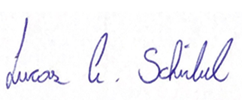
\includegraphics{./figuras/assinatura.png} \\[5.0pt]
    \hline \\[-25.0pt]
    Físico Me. Lucas Alexandre Schirbel \\[-7.0pt]
    Pesquisador \\[-7.0pt]
    RE: 117113 \\[0.0pt]
    \hline
  \end{tabular}
  \end{adjustwidth}
\end{table}



\section{COMPLETUDE DOS DADOS}

\begin{figure}[htb!]
    \centering
	\captionsetup{justification=raggedright, singlelinecheck=false, width=1\textwidth}
    \caption{Gráfico de completude dos dados para o mês de MÊS para estação ESTAÇÃO.}
    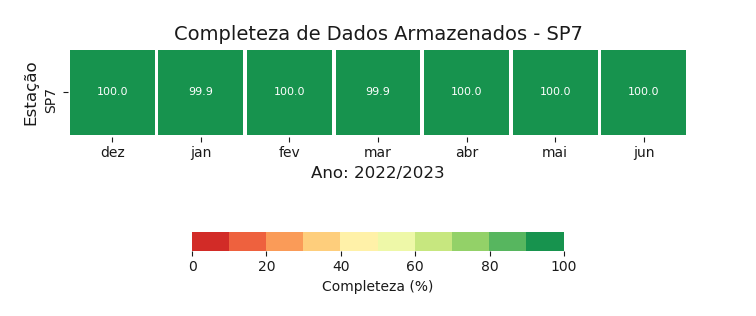
\includegraphics[width=1.0\textwidth]{/home/suporte/projetos/ipt-latex/figuras/completude.png} % Substitua pelo nome da imagem e ajuste o tamanho
    \caption*{Fonte: IPT}
    \label{fig:completude}
\end{figure}



\section{TABELA DE EVENTOS}
\begin{center}
\scriptsize
\setlength{\arrayrulewidth}{0.05pt}
\begin{longtable}{ccccS[table-format=6.0]S[table-format=7.0]ccc}
\captionsetup{justification=justified,singlelinecheck=false}
\caption{Listagem de eventos detectados e categorizados durante o período de interesse.\\ A coluna \textit{Cat} representaria a categoria na qual o evento foi classificado sendo \textit{Q} = Detonação/Desmontes, \textit{E} = Sismo Regional e \textit{I} = Sismo induzido e \textit{N} = Não-localizável. O valor da energia para os sismos foi obtido a partir da magnitude através da relação proposta por Richter (1958). Fonte: IPT.}\\
%%%%%%%%%%%%%%%%%%%%%%%%%%%%%%%%%%%%%%%%%%%%%%%%%%%%%%%
\hline \\[-4ex]
\hline \\[-5ex]
\multicolumn{1}{c}{ID} &
\multicolumn{1}{c}{Hora de Origem (UTC)} &
\multicolumn{1}{c}{Longitude} &
\multicolumn{1}{c}{Latitude} &
\multicolumn{1}{c}{UTM X} &
\multicolumn{1}{c}{UTM Y} &
\multicolumn{1}{c}{MLv} &
\multicolumn{1}{c}{Energia} &
\multicolumn{1}{c}{Cat} \\


\\[-5.0ex] \hline
\\[-5.0ex]

\multicolumn{1}{c}{\textit{{}}} & 
\multicolumn{1}{c}{\textit{{}}} & 
\multicolumn{1}{c}{\textit{(\textdegree\hspace{0.25em})}} & 
\multicolumn{1}{c}{\textit{(\textdegree\hspace{0.25em})}} & 
\multicolumn{1}{c}{\textit{{(m)}}} & 
\multicolumn{1}{c}{\textit{{(m)}}} & 
\multicolumn{1}{c}{\textit{{}}} & 
\multicolumn{1}{c}{\textit{{(J)}}} & 
\multicolumn{1}{c}{\textit{{}}} \\ 

\\[-5.0ex] \hline
\\[-4.0ex]
\endfirsthead


%%%%%%%%%%%%%%%%%%%%%%%%%%%%%%%%%%%%%%%%%%%%%%%%%%%%%%%
\hline \\[-4ex]
\hline \\[-5ex]
\multicolumn{1}{c}{ID} &
\multicolumn{1}{c}{Hora de Origem (UTC)} &
\multicolumn{1}{c}{Longitude} &
\multicolumn{1}{c}{Latitude} &
\multicolumn{1}{c}{UTM X} &
\multicolumn{1}{c}{UTM Y} &
\multicolumn{1}{c}{MLv} &
\multicolumn{1}{c}{Energia} &
\multicolumn{1}{c}{Cat} \\


\\[-5.0ex] \hline
\\[-5.0ex]

\multicolumn{1}{c}{\textit{{}}} & 
\multicolumn{1}{c}{\textit{{}}} & 
\multicolumn{1}{c}{\textit{(\textdegree\hspace{0.25em})}} & 
\multicolumn{1}{c}{\textit{(\textdegree\hspace{0.25em})}} & 
\multicolumn{1}{c}{\textit{{(m)}}} & 
\multicolumn{1}{c}{\textit{{(m)}}} & 
\multicolumn{1}{c}{\textit{{}}} & 
\multicolumn{1}{c}{\textit{{(J)}}} & 
\multicolumn{1}{c}{\textit{{}}} \\

\\[-5.0ex] \hline
\\[-4.0ex]
\endhead
\hline
\caption*{Fonte: IPT.}

\endlastfoot
%%%%%%%%%%%%%%%%%%%%%%%%%%%%%%%%%%%%%%%%%%%%%%%%%%%%%%%
MC\_20230929\_145625 & 2023-09-29T14:56:25 & -51,4254 & -27,5585 & 458002 & 6951629 & -0,4 & \num[round-precision=3,round-mode=figures,scientific-notation=true]{138.954} & I \\
MC\_20230929\_111457 & 2023-09-29T11:14:57 & -51,4355 & -27,5698 & 457015 & 6950377 & -0,1 & \num[round-precision=3,round-mode=figures,scientific-notation=true]{563.721} & I \\
MC\_20230929\_103129 & 2023-09-29T10:31:29 & -51,4330 & -27,5814 & 457259 & 6949094 & -0,1 & \num[round-precision=3,round-mode=figures,scientific-notation=true]{432.42} & I \\
MC\_20230929\_100122 & 2023-09-29T10:01:22 & -51,4258 & -27,5814 & 457970 & 6949092 & -0,0 & \num[round-precision=3,round-mode=figures,scientific-notation=true]{690.793} & I \\
MC\_20230927\_124624 & 2023-09-27T12:46:24 & -51,3295 & -27,6895 & 467507 & 6937149 & -0,4 & \num[round-precision=3,round-mode=figures,scientific-notation=true]{127.28} & I \\
MC\_20230919\_025258 & 2023-09-19T02:52:58 & -51,3256 & -27,7085 & 467895 & 6935043 & -1,0 & \num[round-precision=3,round-mode=figures,scientific-notation=true]{8.46601} & I \\
MC\_20230916\_152149 & 2023-09-16T15:21:49 & -50,5896 & -27,9284 & 540376 & 6910658 & 1,1 & \num[round-precision=3,round-mode=figures,scientific-notation=true]{82262.6} & Q \\
MC\_20230906\_151824 & 2023-09-06T15:18:24 & -51,8444 & -28,0489 & 417013 & 6897088 & 1,7 & \num[round-precision=3,round-mode=figures,scientific-notation=true]{1.17607e+06} & Q \\
MC\_20230906\_121305 & 2023-09-06T12:13:05 & -51,3376 & -27,7136 & 466720 & 6934480 & -0,6 & \num[round-precision=3,round-mode=figures,scientific-notation=true]{60.8546} & I \\
MC\_20230904\_002008 & 2023-09-04T00:20:08 & -51,3298 & -27,7133 & 467484 & 6934510 & -0,8 & \num[round-precision=3,round-mode=figures,scientific-notation=true]{23.2406} & I \\
MC\_20230902\_081604 & 2023-09-02T08:16:04 & -51,3007 & -27,7044 & 470355 & 6935509 & -0,7 & \num[round-precision=3,round-mode=figures,scientific-notation=true]{30.4004} & I \\
\end{longtable}
\end{center}



    \newpage
    \section{Mapa de eventos}
    \begin{figure}[ht!]
    \centering
    \captionsetup{justification=justified, singlelinecheck=false, width=1\textwidth}
    \caption{Mapa da região de interesse no entorno do empreendimento, mostrando as principais cidades, rodovias e rios, com a localização das pedreiras, estações \textbf{BCM2} e \textbf{MC9}, e eventos próximos ao empreendimento detectados no período de interesse.}
    \begin{mdframed}[
        linecolor=black,
        linewidth=1pt,
        roundcorner=10pt,
    ]
    \begin{center}
    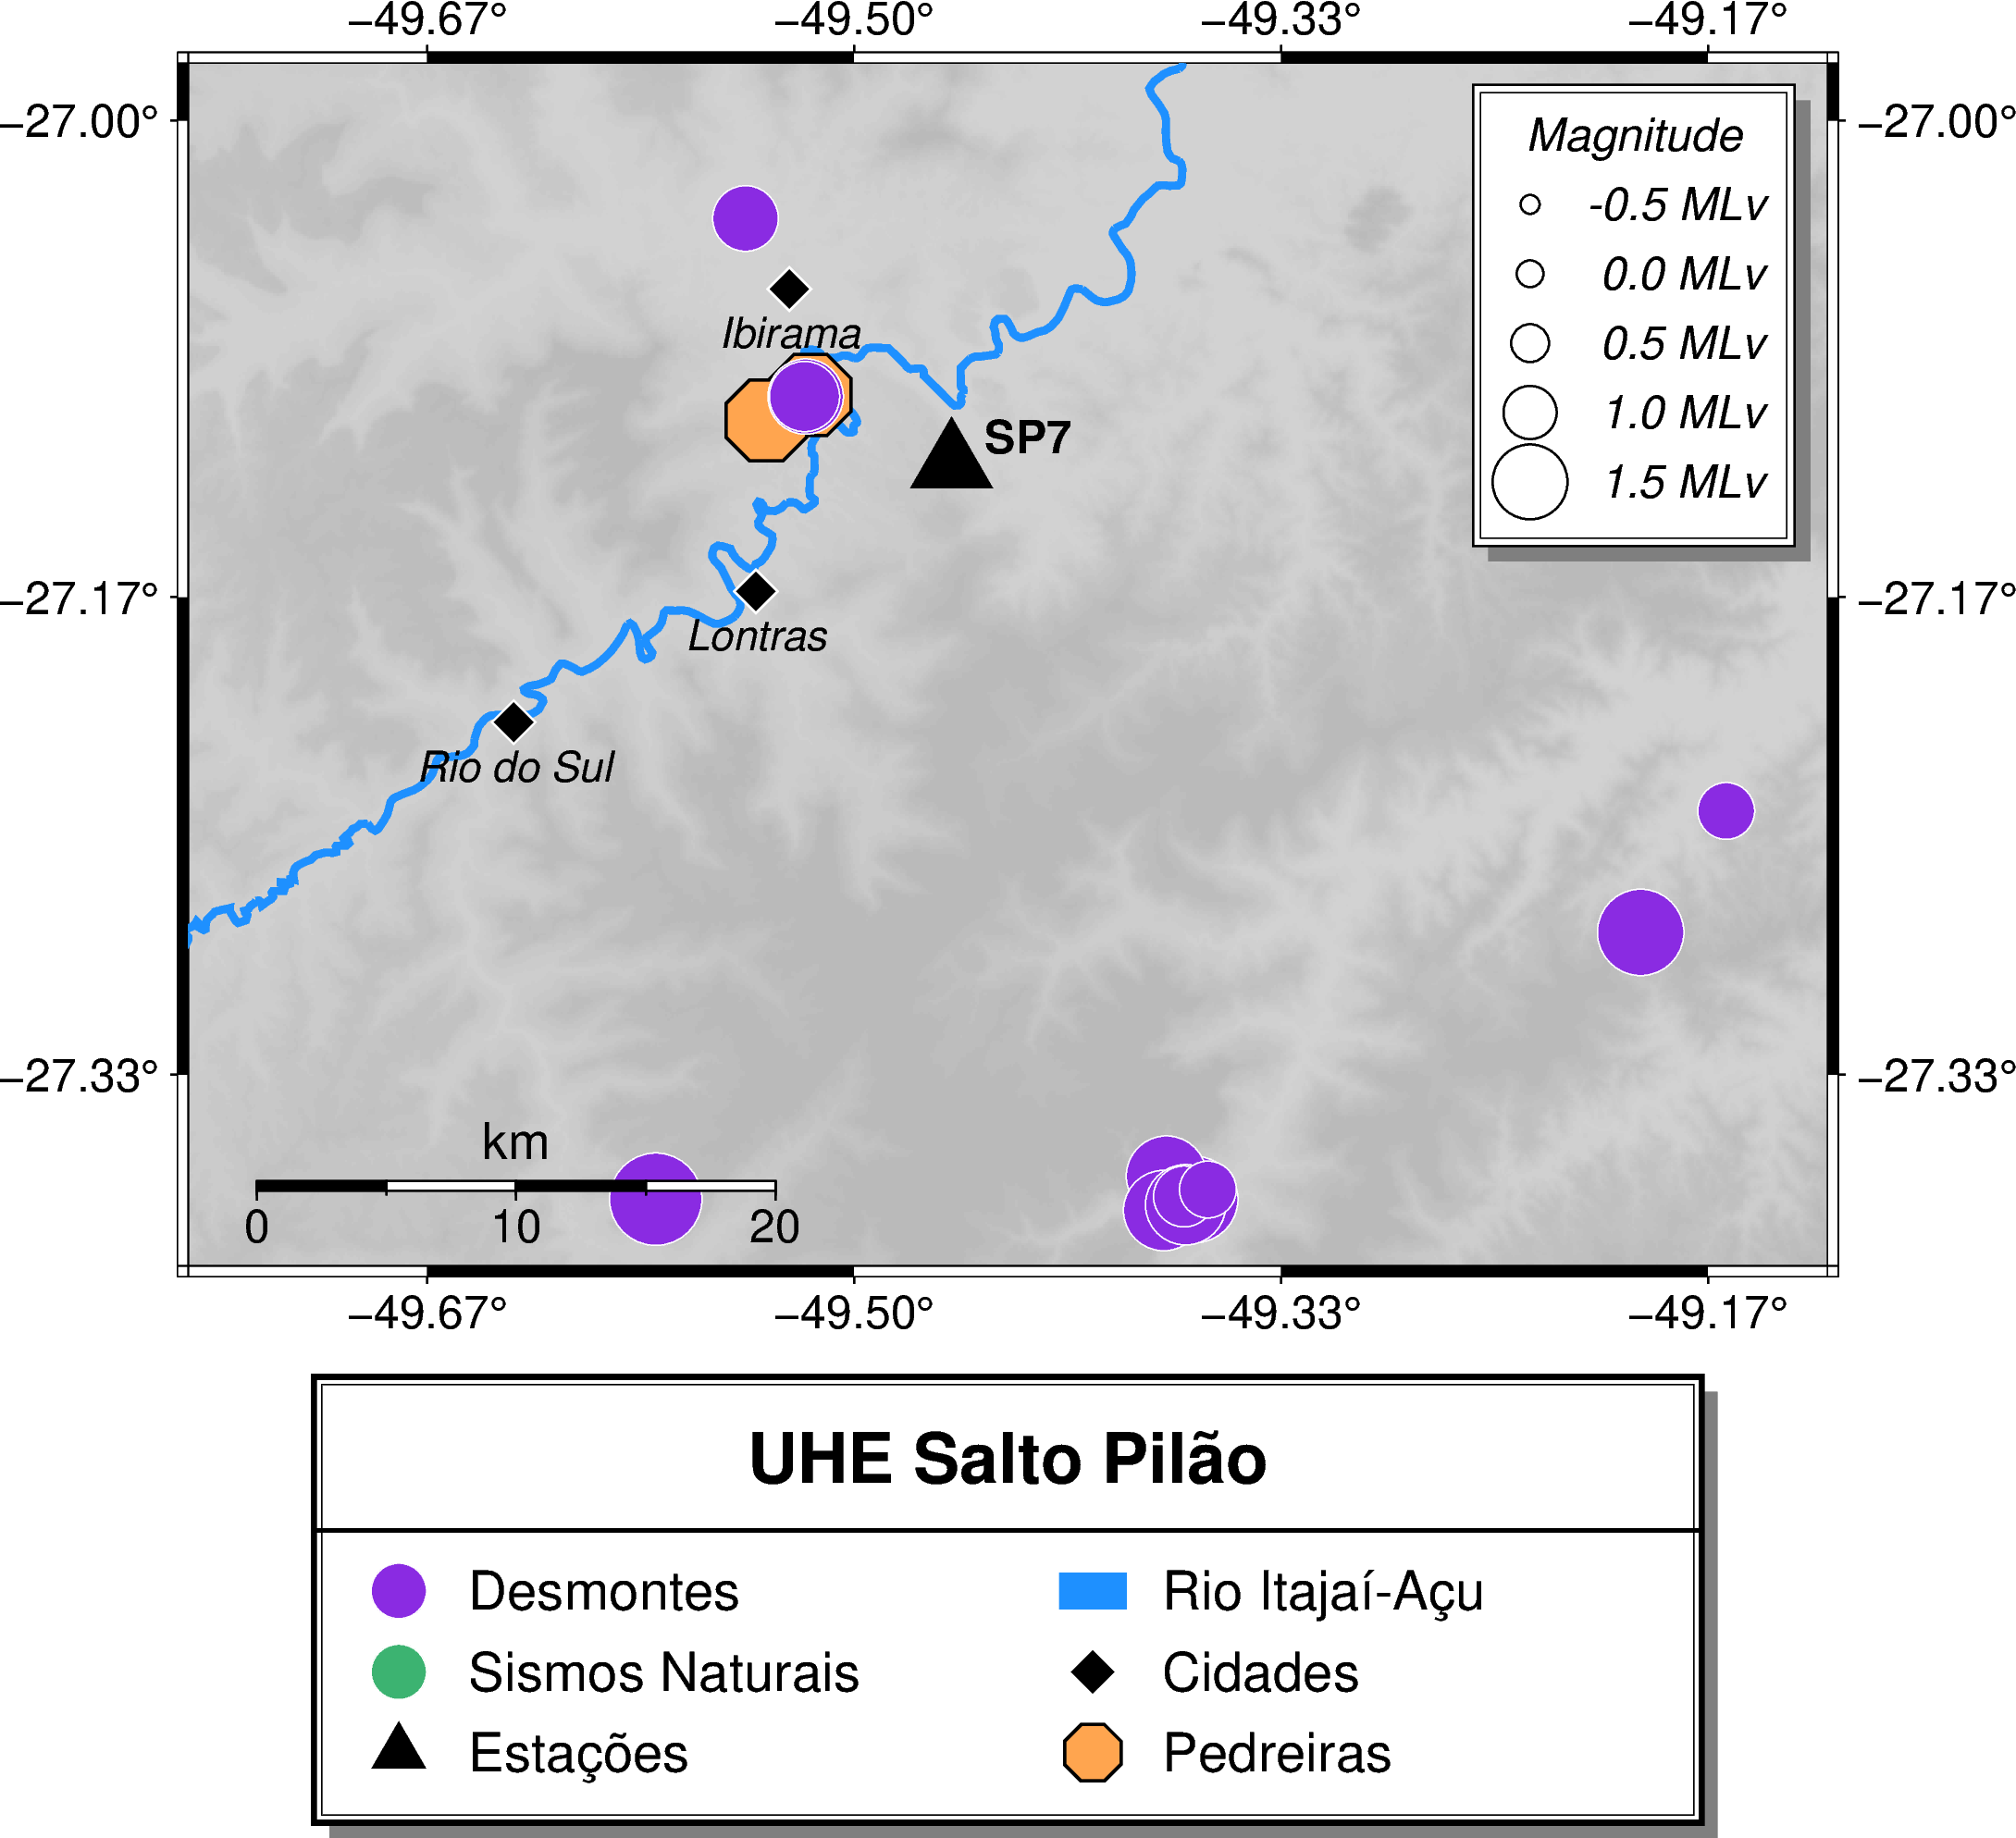
\includegraphics[width=1.0\textwidth]{./machadinho/figuras/mapaevents.png}
    \end{center}
    \end{mdframed}
    \caption*{Fonte: IPT}
    \end{figure}
    \newpage
    


% Bibliografia
\clearpage
\section{REFERÊNCIAS BIBLIOGRÁFICAS}

C. F. RICHTER, \textit{Elementary Seismology}, W. H. Freeman and Co., San Francisco, 1958, 768 pp.
%\renewcommand{\refname}{REFERÊNCIAS}
%\addcontentsline{toc}{section}{REFERÊNCIAS}
%\bibliography{ref}

\end{document}
